\documentclass[letterpaper,12pt,titlepage]{article}

\usepackage[utf8]{inputenc} 
\usepackage[T1]{fontenc}    
\usepackage[spanish,mexico]{babel}


% paquetes que te pueden ser de utilidad
\usepackage[paper=portrait,pagesize]{typearea}
\usepackage{listings}
\usepackage{comment}
\usepackage{enumerate}
\usepackage{wrapfig}
\usepackage{amsmath}	
\DeclareMathOperator*{\argmax}{argmax}
\usepackage{amssymb}		
\usepackage{amsfonts}
\usepackage{latexsym}
\usepackage{textcomp}
\usepackage{stmaryrd}
\usepackage{layout}
\usepackage{float}
\usepackage{dsfont}
\usepackage[dvipsnames]{xcolor}
\usepackage{graphicx} 
\usepackage{wasysym}
\usepackage{marvosym}
\usepackage{rotating}
\usepackage{hyperref}
\usepackage{setspace}
\usepackage{scrextend}
\usepackage{caption} 
\usepackage{pifont}
\usepackage{booktabs}
\usepackage{tikz,pgfplots}
\usepackage{enumitem}
\usepackage{multicol}
\usepackage[edges]{forest}
\usetikzlibrary{arrows.meta}
\usetikzlibrary{shapes,calc}
\usepackage{xcolor}

\newtheorem{defi}{Definición} %Formato definiciones
\newtheorem{teo}{Teorema} %Formato teoremas
\newtheorem{lem}{Lema} %Formato teoremas
\newtheorem{algo}{Algoritmo} %Formato teoremas

\tikzstyle{blueV}=[circle, fill=blue, draw,
                   minimum size=6pt, line width=0.75pt,
                   inner sep=0pt, outer sep=0pt]
\tikzstyle{yellowV}=[circle, fill=yellow, draw,
                  minimum size=6pt, line width=0.75pt,
                  inner sep=0pt, outer sep=0pt]
\tikzstyle{vertex}=[circle, draw, minimum size=6pt,
                    line width=0.75pt, inner sep=0pt,
                    outer sep=0pt]
\newcommand*\circled[1]{\tikz[baseline=(char.base)]{
            \node[shape=circle,draw,inner sep=2pt] (char) {#1};}}
\newcommand{\sep}{\hspace*{.5em}}

% márgenes

\usepackage[lmargin=1.5cm,rmargin=1.5cm,top=2cm,bottom=2cm,headsep=2cm,headheight=20pt]{geometry}

\title{}
\author{}
\date{}

\onehalfspacing
\allowdisplaybreaks

\begin{document}

\begin{titlepage}
\begin{flushleft}																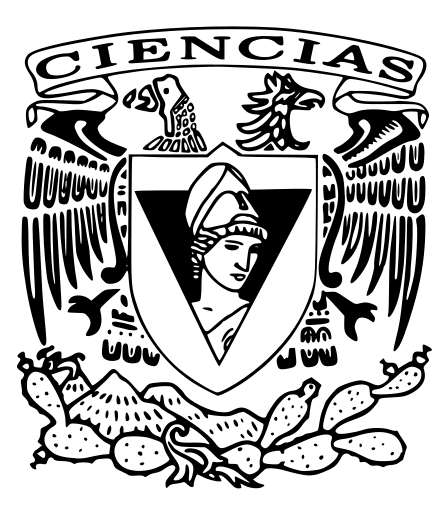
\includegraphics[scale = 0.20]{FC (1).png} \hfill 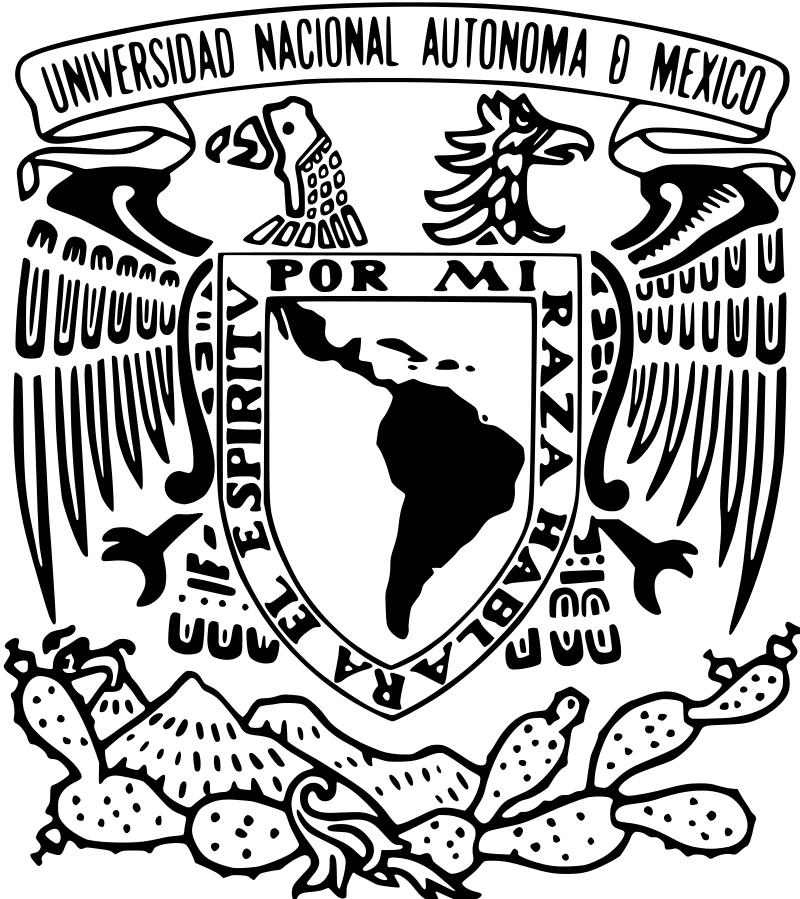
\includegraphics[scale = 0.10]{UNAM (1).png}
\end{flushleft}
    \begin{center}
    {\large \textsc{Compiladores 2025-1}}
\end{center}
\begin{table}[h]
 \centering
\begin{tabular}{r l}
 \small \bfseries Profesora: & \hspace{-0.4cm} \small Ariel Adara Mercado Martínez\\
 \small \bfseries Ayudante: & \hspace{-0.4cm} \small Carlos Gerardo Acosta Herández\\
\end{tabular}
\end{table}

\begin{center}
\large{\textbf{Práctica 3: Implementación de un Analizador Sintáctico de descenso recursivo.)}}
\end{center}


\begin{center}
\begin{tabular}{c c}
   \textbf{Nombre}  & \textbf{No. de Cuenta} \\
    Vázquez Torrijos Damián & 318309877\\
    
\end{tabular}
\end{center}
\vspace*{1cm}%%%
\begin{center}
    \textbf{\large{26 de Septiembre del 2024}}
\end{center}

\end{titlepage}

Para comodidad, se abreviaron las producciones:
\begin{itemize}
    \item programa $=$ $Pr$
    \item declaraciones $=$ $Ds$
    \item declaracion $=$ $D$
    \item tipo $=$ $T$
    \item lista\_var $=$ $L\_V$
    \item sentencias $=$ $Ss$
    \item sentencia $=$ $S$
    \item expresion $=$ $E$
\end{itemize}

\begin{enumerate}
{\bfseries \item \boldmath Determinar los conjuntos $N$, $\Sigma$ y el símbolo inicial $S$.}
\begin{itemize}
    {\bfseries \item \boldmath $N = $} $\{Pr, Ds, D, Ss, S, T, L\_V, E\}$
    {\bfseries \item \boldmath $\Sigma = $} $\{;, id, =, if, else, while, +, -, *, /, (, ), num\}$
    {\bfseries \item \boldmath $S = $} $\{Pr\}$
\end{itemize}
{\bfseries \item \boldmath Mostrar el proceso de eliminación de ambigüedad o justificar, en caso de no ser necesario.}

La producción $E$ tiene ambigüedad, para eliminarla debemos definir el orden de procedencia de los operadores de menor a mayor:
\begin{itemize}
    \item $-$
    \item $+$
    \item $/$
    \item $*$
    \item $()$
\end{itemize}
Una vez definido el orden, hacemos nuevas producciones en base al algoritmo de la eliminación de ambigüedad:
\begin{itemize}
    \item $E\rightarrow E-F|F$
    \item $F\rightarrow F+G|G$
    \item $G\rightarrow G/H|H$
    \item $H\rightarrow H*I|I$
    \item $I\rightarrow (E)|id|num$
\end{itemize}
{\bfseries \item \boldmath 
Mostrar el proceso de eliminación de la recursividad izquierda o justificar, en caso de no ser necesario.}

Las producciones $Ds, L\_V, Ss, E, F, G, H$ tienen recursividad izquierda, por lo que hacemos nuevas producciones en base al algoritmo de la eliminación de la recursividad izquierda:
\begin{itemize}
    \item $Ds\rightarrow D Ds'$\\
    $Ds'\rightarrow D Ds'|\epsilon$
    \item $L\_V\rightarrow id L\_V'$\\
    $L\_V'\rightarrow ,id L\_V'|\epsilon$
    \item $Ss\rightarrow S Ss'$\\
    $Ss'\rightarrow S Ss'|\epsilon$
    \item $E\rightarrow F E'$\\
    $E'\rightarrow -F E'|\epsilon$
    \item $F\rightarrow GF'$\\
    $F'\rightarrow +G F'|\epsilon$
    \item $G\rightarrow H G'$\\
    $G'\rightarrow /H G'|\epsilon$
    \item $H\rightarrow I$\\
    $H'\rightarrow *I H'|\epsilon$
\end{itemize}
{\bfseries \item \boldmath Mostrar el proceso de factorización izquierda o justificar, en caso de no ser necesario.}

No hay producciones que se puedan factorizar debido a que no son de la forma $A\rightarrow\alpha\beta_1|\alpha\beta_2|\alpha\beta_3|\ldots\\|\alpha\beta_n|\gamma_1|\gamma_2|\ldots|\gamma_n$, es decir, no tienen prefijo en común.
{\bfseries \item \boldmath Mostrar los nuevos conjuntos $N$ y $P$.}
\begin{itemize}
    {\bfseries \item \boldmath $N = $} $\{Pr, Ds, Ds', D, T, L\_V, L\_V', Ss, Ss', S, E, E', F, F', G, G', H, H', I\}$
    {\bfseries \item \boldmath $P = $} $\{Pr\rightarrow Ds Ss\\ Ds\rightarrow D Ds'\\
    Ds'\rightarrow D Ds'|\epsilon\\
    D\rightarrow T L\_V;\\
    T\rightarrow int|float\\
    L\_V\rightarrow id L\_V'\\
    L\_V'\rightarrow ,id L\_V' |\epsilon\\
    Ss\rightarrow S Ss\\
    Ss'\rightarrow S Ss'|\epsilon\\
    S\rightarrow id = E;|if(E) Ss else Ss|while(E) Ss\\
    E\rightarrow F E'\\
    E'\rightarrow -F E'|\epsilon\\
    F\rightarrow G F'\\
    F'\rightarrow +G F'|\epsilon\\
    G\rightarrow H G'\\
    G'\rightarrow /H G'|\epsilon\\
    H\rightarrow I H'\\
    H'\rightarrow *I H'|\epsilon\\
    I\rightarrow (E)|id|num\}$
\end{itemize}
\end{enumerate}



\end{document}
